\fancyhead{}
\fancyfoot{}


\lhead{Configurar VPN}

\section{Configuraci�n de VPN}

La especificaci�n para PPTP fue publicada por el RFC 2637\cite{rfc:2637}, aunque no ha sido ratificada como est�ndar por el IETF.\\

Point-To-Point Tunneling Protocol (\Gls{pptp}) permite el intercambio seguro de datos de un cliente a un servidor formando una Red Privada Virtual (VPN, por el anglicismo Virtual Private Network), basado en una red de trabajo v�a \Gls{tcp/ip}. El punto fuerte del PPTP es su habilidad para proveer en la demanda, multi-protocolo soporte existiendo una infraestructura de �rea de trabajo, como INTERNET. Esta habilidad permitir� a una compa��a usar Internet para establecer una red privada virtual (VPN) sin el gasto de una l�nea alquilada.
 
Escoger el men� \textbf{New Terminal} $\rightarrow$  \textbf{system-reset} \\
\subsection{Configuraci�n VPN Server} 
\begin{figure}[H]
\begin{center}
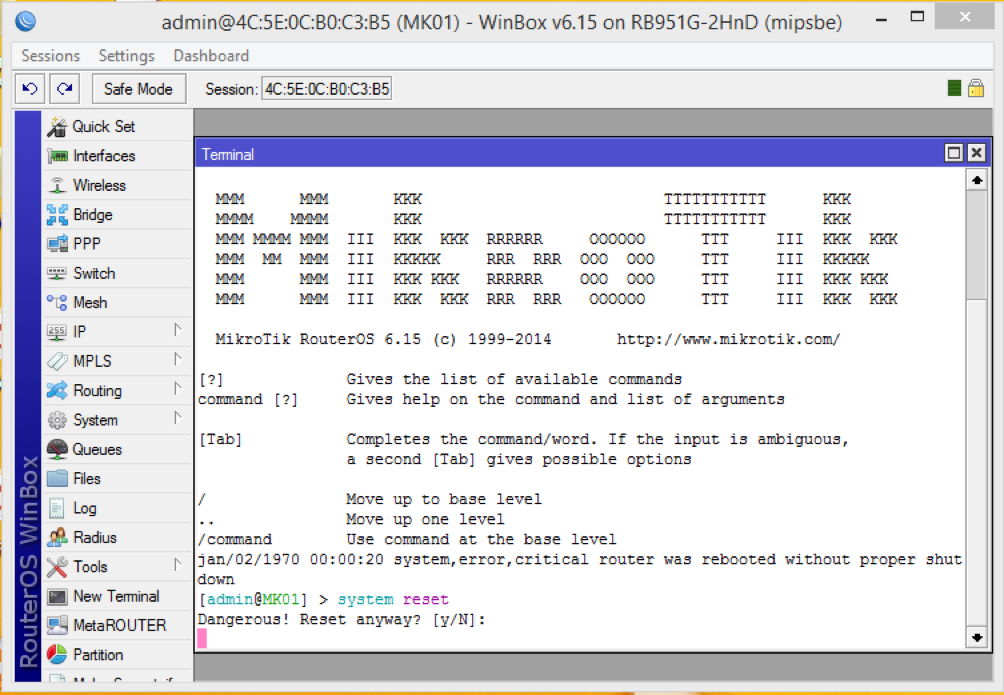
\includegraphics[scale = .5]{./figuras/figura081.png}
\caption{Restaurar configuraciones MK1}
\label{restaurar-configuraciones-mk1}
\end{center}
\end{figure}

 Escoger el men� \textbf{Mac Address} $\rightarrow$  \textbf{Connect}\\
\begin{figure}[H]
\begin{center}
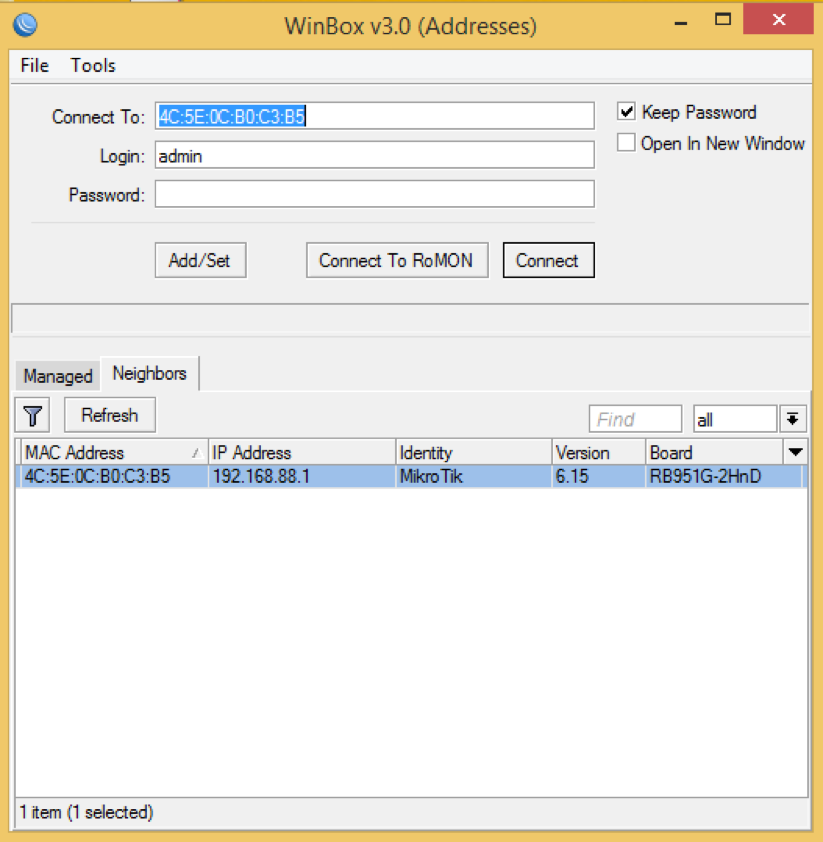
\includegraphics[scale = .5]{./figuras/figura082.png}
\caption{Winbox con el MK1 ya con las configuraciones de fabrica}
\label{Winbox-mk1-configuraciones-fabrica}
\end{center}
\end{figure}
 
Escoger el men� \textbf{Remove Configuration} \\
\begin{figure}[H]
\begin{center}
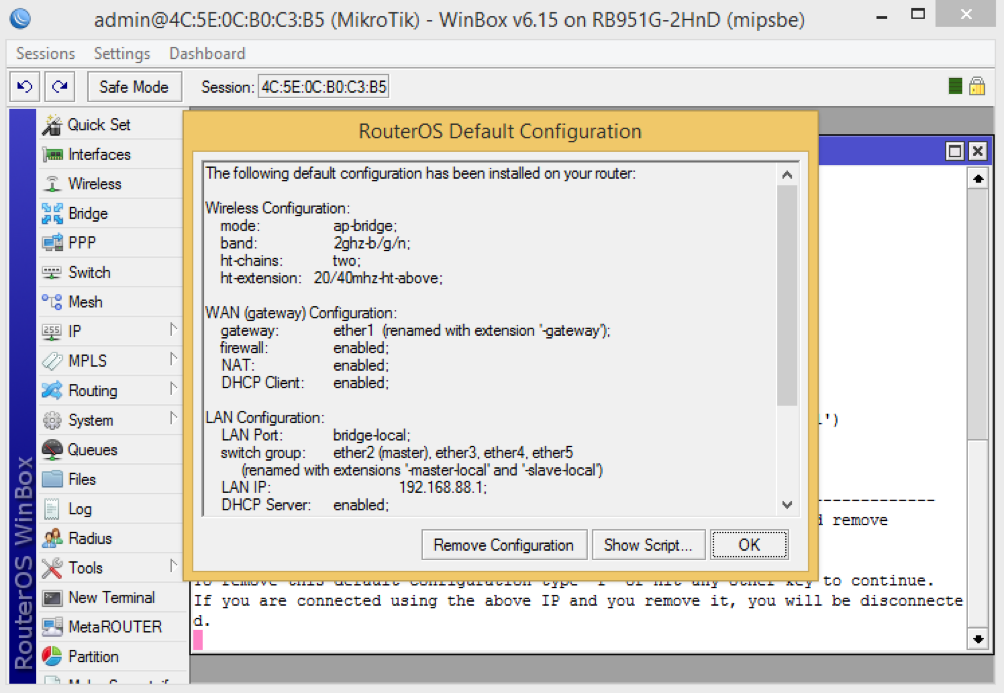
\includegraphics[scale = .5]{./figuras/figura083.png}
\caption{Remover configuraciones}
\label{remover-configuraciones-83}
\end{center}
\end{figure}

Escoger el men� \textbf{IP} $\rightarrow$  \textbf{Address}  $\rightarrow$ \textcolor{red}{\textbf{+}}\\
\begin{figure}[H]
\begin{center}
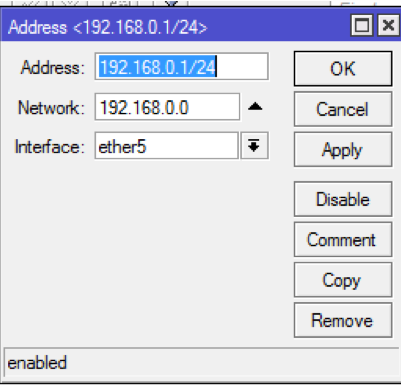
\includegraphics[scale = .5]{./figuras/figura084.png}
\caption{Configurar IP}
\label{configurar-ip-84}
\end{center}
\end{figure}

 Escoger el men� \textbf{Wireless} $\rightarrow$  \textbf{wlan1}  $\rightarrow$ \textbf{Wireless}\\
\begin{figure}[H]
\begin{center}
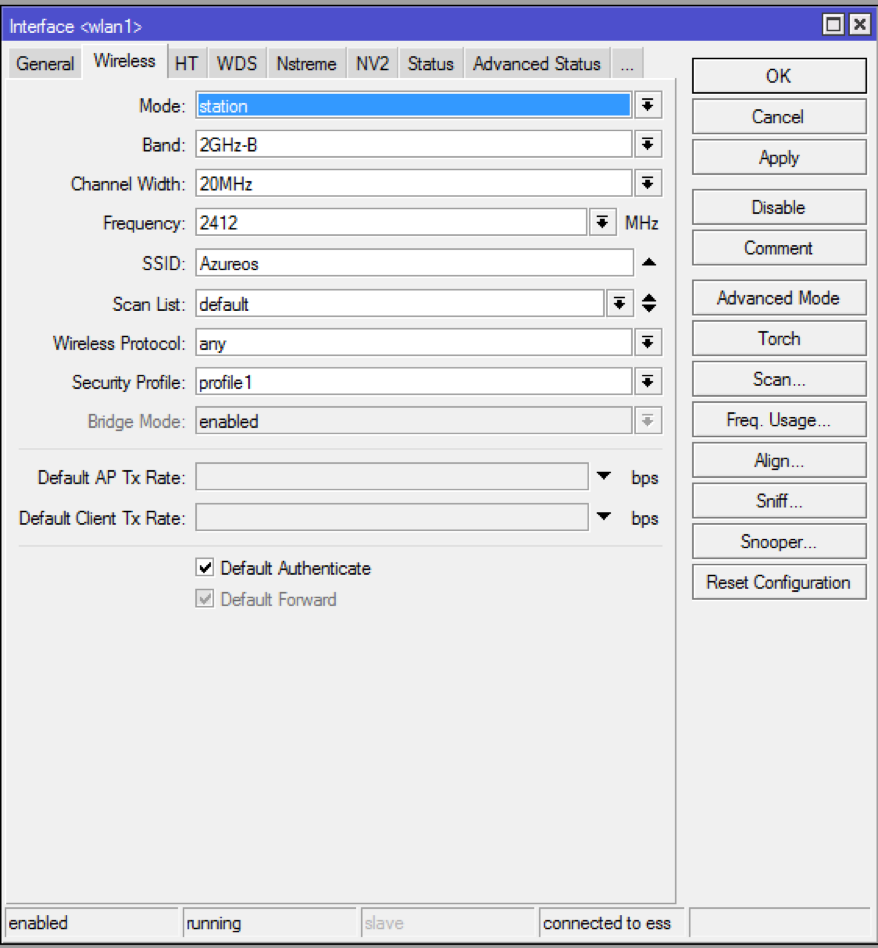
\includegraphics[scale = .5]{./figuras/figura085.png}
\caption{Conectar al WIFI del Celular}
\label{conectar-wifi-celular-85}
\end{center}
\end{figure}

 Escoger el men� \textbf{Wireless} $\rightarrow$  \textbf{Security Profiles}  $\rightarrow$ \textcolor{red}{\textbf{+}}\\
\begin{figure}[H]
\begin{center}
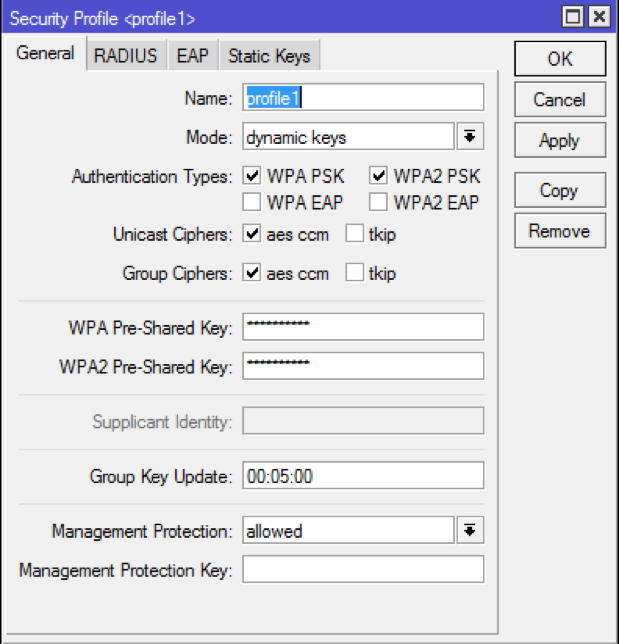
\includegraphics[scale = .5]{./figuras/figura086.png}
\caption{Configuraciones de Seguridad del WIFI}
\label{confi-seguridad-wifi-86}
\end{center}
\end{figure}
 
\begin{figure}[H]
\begin{center}
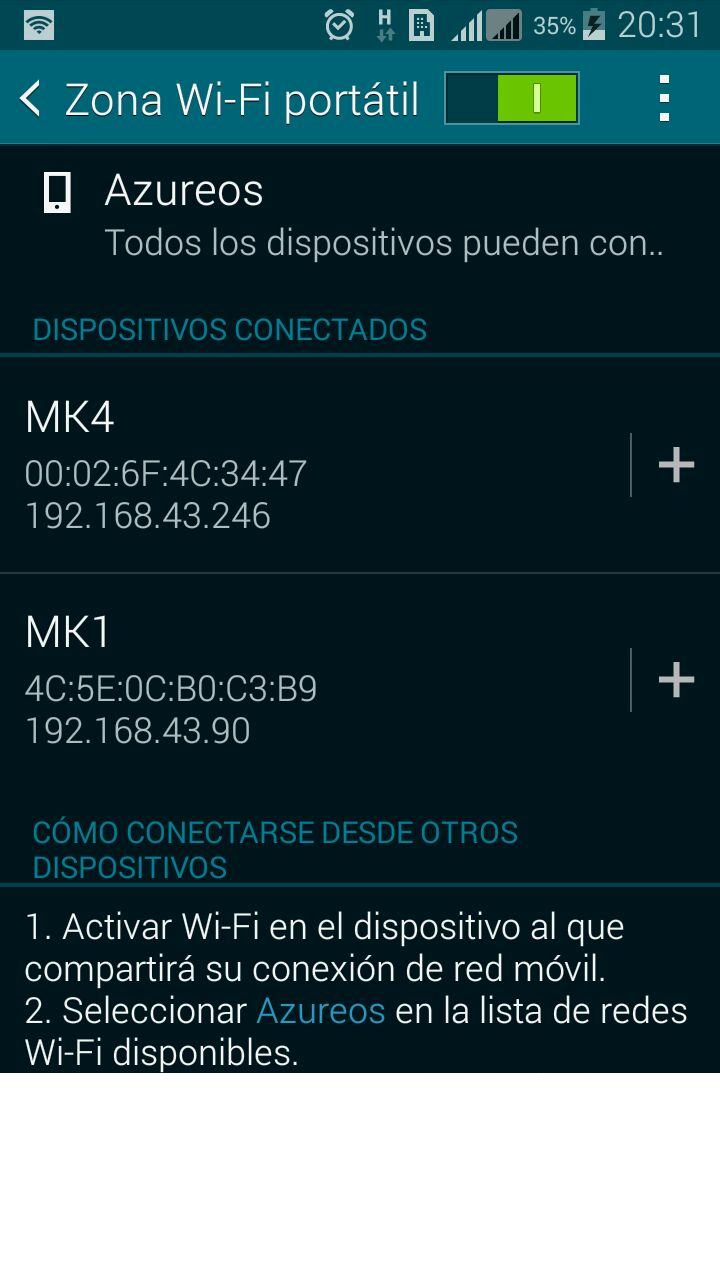
\includegraphics[scale = .3]{./figuras/figura102.png}
\caption{MK1 y MK4 conectado al Celular}
\label{mk-conectado-cel}
\end{center}
\end{figure}
 

Habilitamos el PPTP Server, para eso nos vamos a la opcion de /PPP Interface; acemos clic e el boton PPTP Server hacemos click en Enabled y en default Profile escogemos default-encryptation. Aplicamos, de esta forma estamos hablilitando al servidor para que permita coneccione PPTP.

Escoger el men� \textbf{PPP} $\rightarrow$  \textbf{PPTP-Server} \\
\begin{figure}[H]
\begin{center}
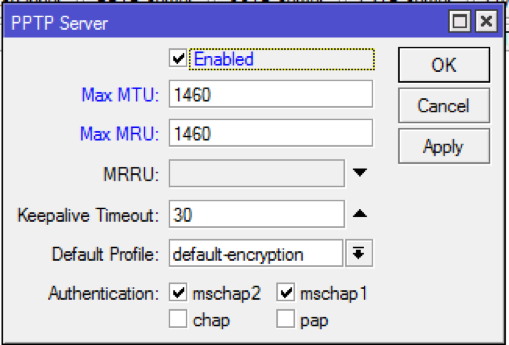
\includegraphics[scale = .5]{./figuras/figura087.png}
\caption{Habilitar Server PPTP}
\label{habilitar-server-pptp}
\end{center}
\end{figure}
 
Ahora agregamos nuestros Clientes VPN, Para eso nos vamos a la pesta�a Secrets, y agregamos los usuarios que sean necesarios.\\

\textbf{Name:} Nombre de Usuario VPN\\
\textbf{Password:} Contrase�a del Usuario VPN\\
\textbf{Service:} Tipo de Protocolo que usara el cliente para su coneccion con el servidor.\\
\textbf{Profile:} Perfil de encryptacion \\
\textbf{Local Address:} Direcci�n IP del equipo anfitri�n, del router local (La IP de puerta de enlace de nuestra LAN anfitri�n.)\\
\textbf{Remote address:} Direccion IP con la cual el equipo cliente se identificara en nuestra re LAN.\\

Escoger el men� \textbf{ppp} $\rightarrow$  \textbf{Secret}  $\rightarrow$ \textcolor{red}{\textbf{+}}\\
\begin{figure}[H]
\begin{center}
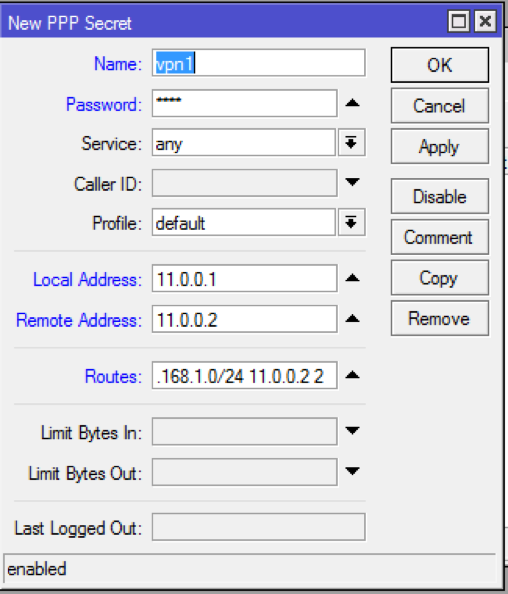
\includegraphics[scale = .5]{./figuras/figura088.png}
\caption{Crear usuario para T�nel por medio del Enlace}
\label{usuario-tunel-enlace}
\end{center}
\end{figure}

Escoger el men� \textbf{ppp} $\rightarrow$  \textbf{Secret}  $\rightarrow$ \textcolor{red}{\textbf{+}}\\
\begin{figure}[H]
\begin{center}
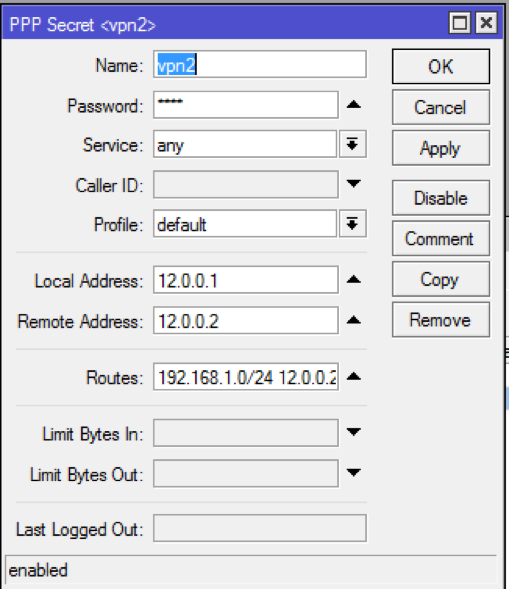
\includegraphics[scale = .5]{./figuras/figura089.png}
\caption{Crear usuario para el T�nel por medio de Internet}
\label{usuario-tunel-internet}
\end{center}
\end{figure}

 Escoger el men� \textbf{PPP} $\rightarrow$  \textbf{Interfaces}\\
\begin{figure}[H]
\begin{center}
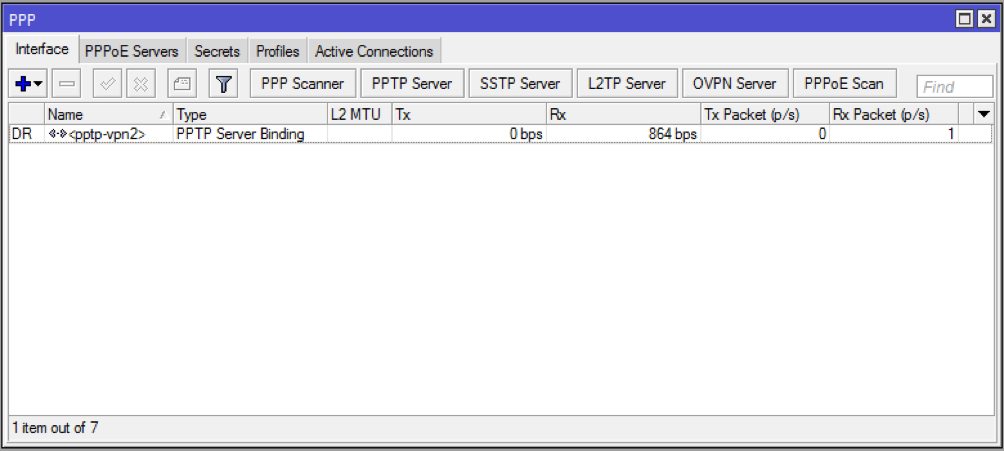
\includegraphics[scale = .5]{./figuras/figura090.png}
\caption{T�nel ya online}
\label{tunel-online}
\end{center}
\end{figure}

 Escoger el men� \textbf{IP} $\rightarrow$  \textbf{Address List}\\
\begin{figure}[H]
\begin{center}
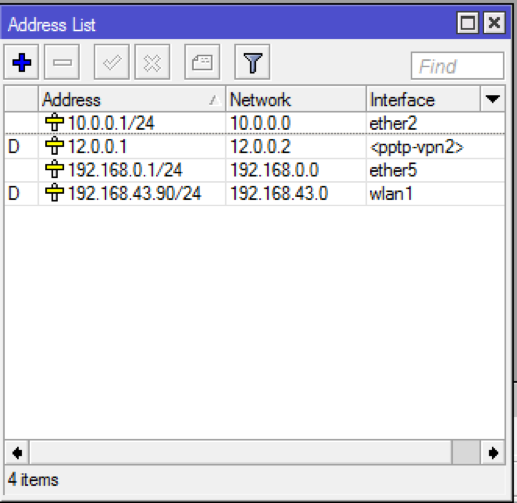
\includegraphics[scale = .5]{./figuras/figura091.png}
\caption{Listado de IP del MK1}
\label{listado-ip-mk1}
\end{center}
\end{figure} 

 \subsection{Configuraci�n VPN Cliente}

Escoger el men� \textbf{New Terminal} $\rightarrow$ \textbf{system reset-configuration}\\
\begin{figure}[H]
\begin{center}
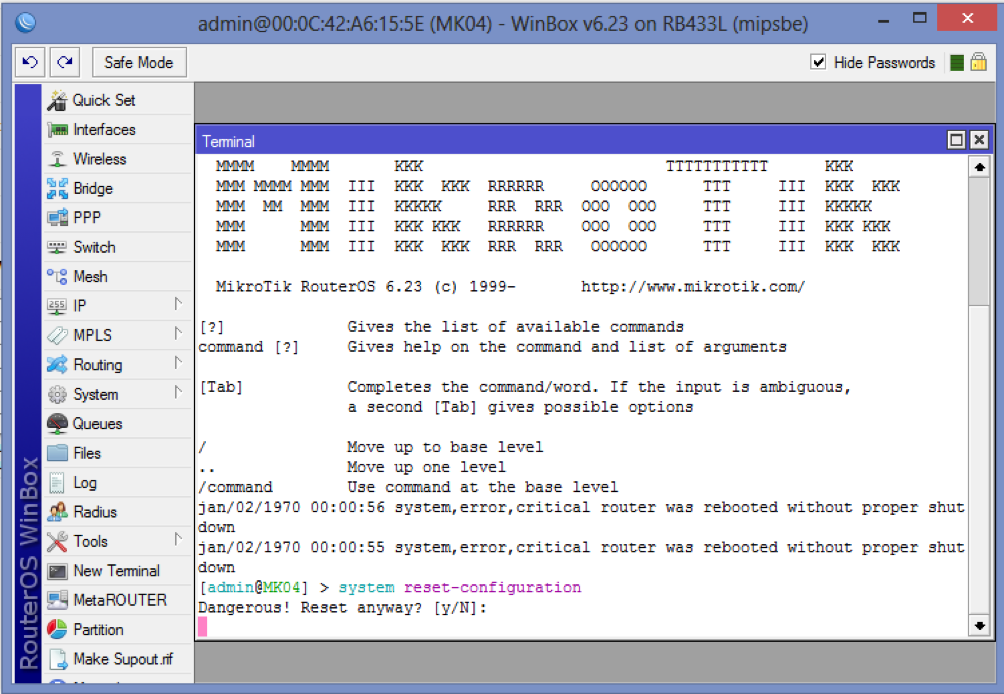
\includegraphics[scale = .5]{./figuras/figura092.png}
\caption{Remover configuraciones}
\label{remover-configuraciones}
\end{center}
\end{figure}
Escoger el men� \textbf{Remove Configuration} \\
\begin{figure}[H]
\begin{center}
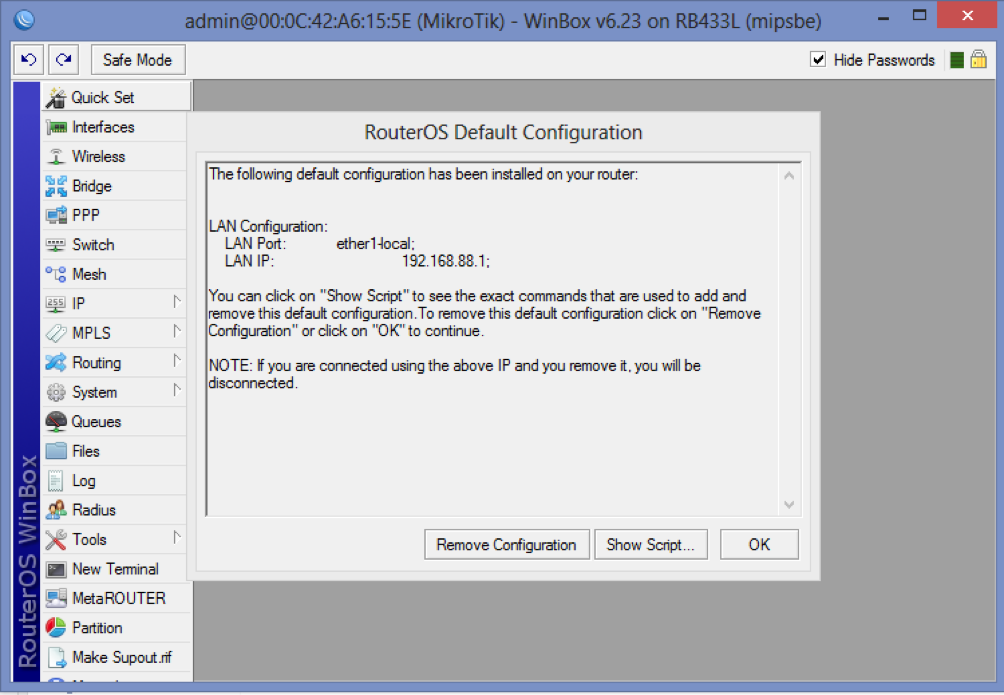
\includegraphics[scale = .5]{./figuras/figura093.png}
\caption{Remover configuraciones por defecto}
\label{remover-configuraciones-defecto}
\end{center}
\end{figure}

Escoger el men� \textbf{Wireless} $\rightarrow$  \textbf{wlan1} $\rightarrow$ \textbf{Wireless}\\
\begin{figure}[H]
\begin{center}
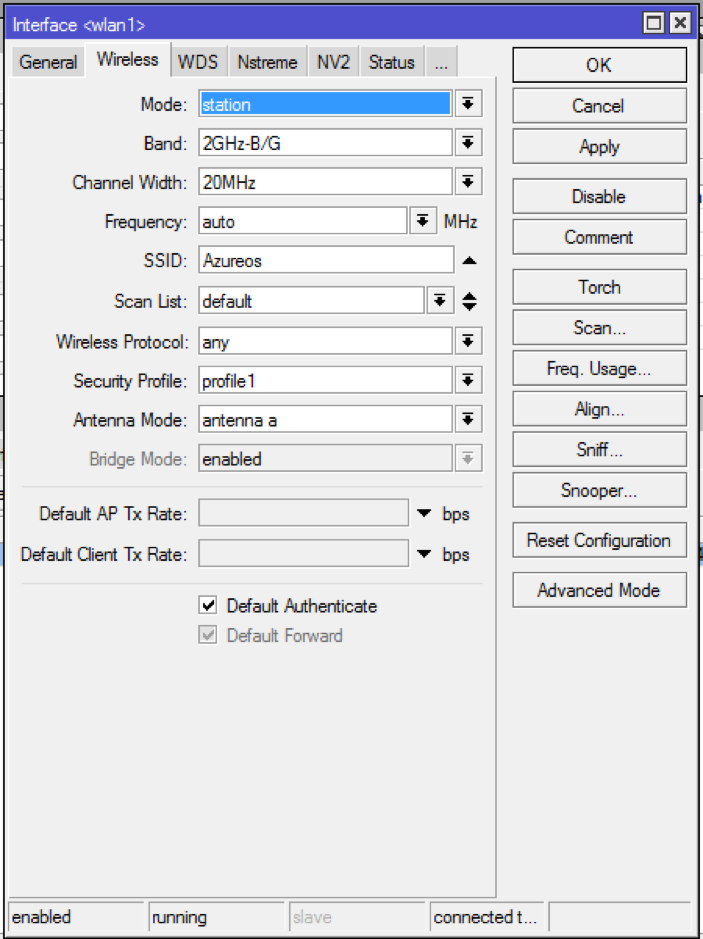
\includegraphics[scale = .5]{./figuras/figura094.png}
\caption{configurar WIFI}
\label{configurar-wifi}
\end{center}
\end{figure}

Escoger el men� \textbf{Wireless} $\rightarrow$  \textbf{Security Profiles}  $\rightarrow$ \textcolor{red}{\textbf{+}}\\

\begin{figure}[H]
\begin{center}
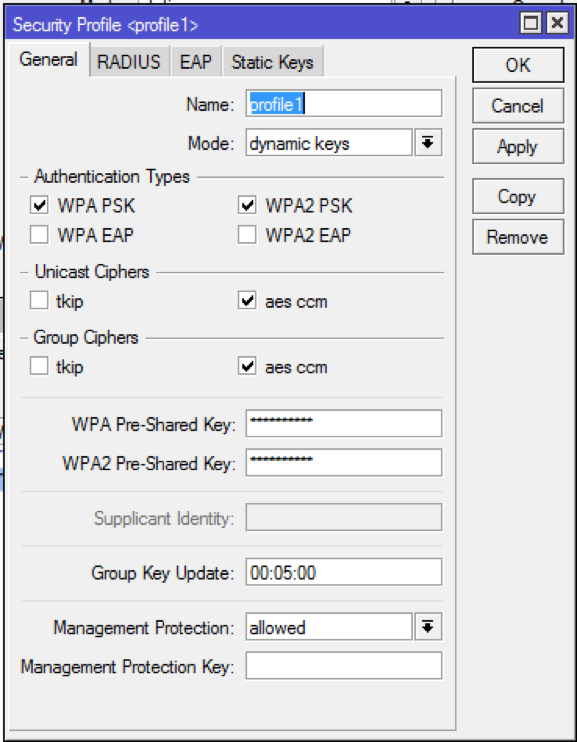
\includegraphics[scale = .5]{./figuras/figura095.png}
\caption{Perfil de seguridad del WIFI}
\label{perfil-seguridad-wifi}
\end{center}
\end{figure}

 Escoger el men� \textbf{IP} $\rightarrow$  \textbf{Address List}  
\begin{figure}[H]
\begin{center}
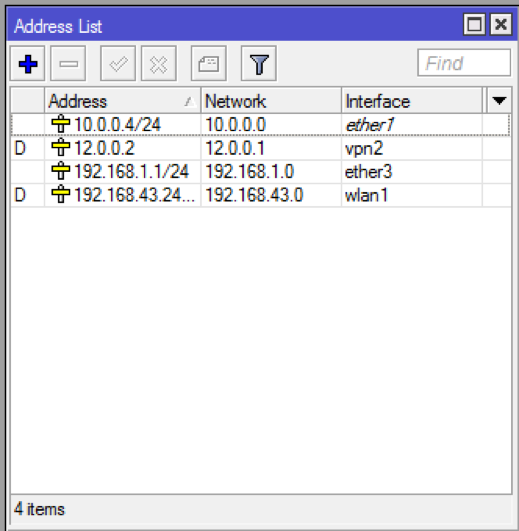
\includegraphics[scale = .5]{./figuras/figura096.png}

\caption{Lista de IP configurado MK4}
\label{lista-ip-configurado-mk4}
\end{center}
\end{figure}
 Escoger el men� \textbf{ppp} $\rightarrow$ \\
\begin{figure}[H]
\begin{center}
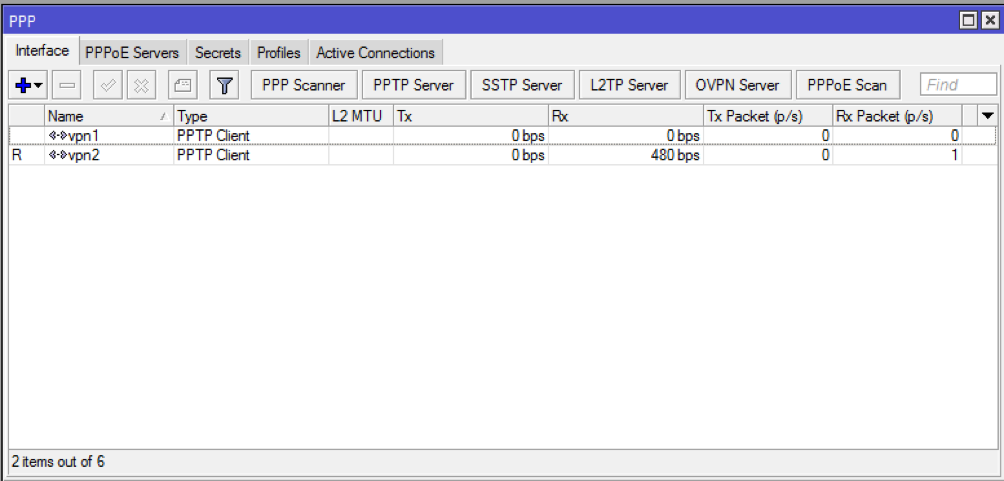
\includegraphics[scale = .5]{./figuras/figura097.png}
\caption{Lista de Discadores Clientes}
\label{lista-discadores-conectado}
\end{center}
\end{figure}

